\begin{figure}[h]
    \begin{small}
        \begin{center}
            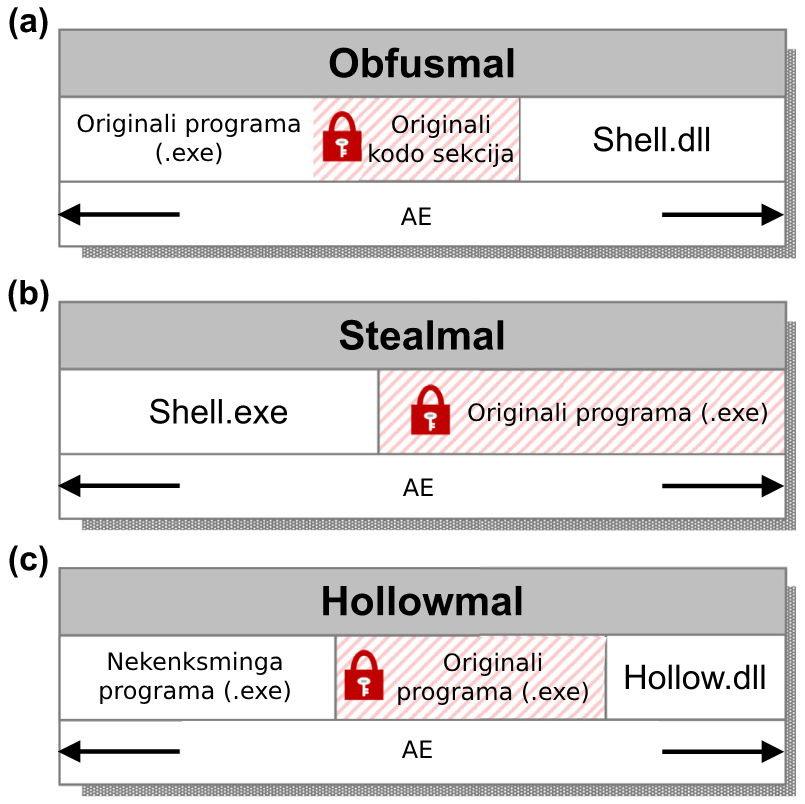
\includegraphics[width=0.95\textwidth]{img/complex-perturbations.png}
        \end{center}
        \caption{Obfusmal (a), Stealmal (b) ir Hollowmal (c) perturbacijų veikimo principų iliustracijos. Adaptuota iš \cite{zhongReinforcementLearningBased2022}}\label{fig:perturbations}
    \end{small}
\end{figure}